% ============================================================
%  Non-Convex Polygon Packing via Simulated Annealing
%  and Bracketing-Bisection Search
%
%  Joel Solis, University of Arizona
%  Applied Mathematics and Numerical Methods, 2026
% ============================================================

\documentclass[10pt]{article}

% ---- Typography ------------------------------------------------
\usepackage{mathptmx}
\usepackage[T1]{fontenc}
\usepackage{microtype}
\linespread{0.96}

% ---- Page layout -----------------------------------------------
\usepackage[
  left=1.65cm, right=1.65cm,
  top=2.6cm,   bottom=2.4cm,
  headheight=13pt, headsep=10pt
]{geometry}
\setlength{\columnsep}{18pt}
\setlength{\columnseprule}{0.35pt}

% ---- Running headers -------------------------------------------
\usepackage{fancyhdr}
\pagestyle{fancy}
\fancyhf{}
\fancyhead[LO]{\small\itshape Non-Convex Polygon Packing via Simulated Annealing}
\fancyhead[RE]{\small\itshape J. Solis}
\fancyhead[RO,LE]{\small\thepage}
\renewcommand{\headrulewidth}{0.4pt}

\fancypagestyle{firstpage}{%
  \fancyhf{}
  \fancyhead[L]{\small\itshape
    Applied Mathematics and Numerical Methods --- University of Arizona, 2026}
  \fancyhead[R]{\small\thepage}
  \renewcommand{\headrulewidth}{0.4pt}%
}

% ---- Section headings ------------------------------------------
\usepackage{titlesec}
\titleformat{\section}[block]
  {\normalfont\bfseries\small\centering}{\thesection.}{0.4em}{\MakeUppercase}
\titleformat{\subsection}[block]
  {\normalfont\itshape\small}{\thesubsection.}{0.4em}{}
\titlespacing*{\section}   {0pt}{7pt plus 2pt minus 1pt}{3pt plus 1pt}
\titlespacing*{\subsection}{0pt}{5pt plus 1pt minus 1pt}{2pt plus 1pt}

% ---- Math and floats -------------------------------------------
\usepackage{amsmath,amssymb}
\usepackage{graphicx}
\usepackage{booktabs,array}
\usepackage[hidelinks]{hyperref}
\usepackage{float}
\usepackage[font=small,labelfont=bf,labelsep=period,
            justification=justified]{caption}
\setlength{\abovecaptionskip}{4pt}
\setlength{\belowcaptionskip}{0pt}
\setcounter{topnumber}{3}
\setcounter{bottomnumber}{2}
\setcounter{totalnumber}{5}
\renewcommand{\topfraction}{0.9}
\renewcommand{\bottomfraction}{0.8}
\renewcommand{\textfraction}{0.07}
\renewcommand{\floatpagefraction}{0.75}
\usepackage{enumitem}
\setlist{noitemsep,topsep=1pt,leftmargin=*}

% ---- Abstract --------------------------------------------------
\usepackage{abstract}
\renewcommand{\abstractname}{}
\renewcommand{\absnamepos}{empty}
\setlength{\absleftindent}{0pt}
\setlength{\absrightindent}{0pt}

% ---- Spacing ---------------------------------------------------
\setlength{\parskip}{2pt}
\setlength{\parindent}{11pt}
\setlength{\abovedisplayskip}{5pt plus 2pt minus 2pt}
\setlength{\belowdisplayskip}{5pt plus 2pt minus 2pt}

% ================================================================
\title{%
  \Large\bfseries
  Non-Convex Polygon Packing via Simulated Annealing\\[4pt]
  and Bracketing-Bisection Search%
}

\author{%
  Joel Solis%
  \thanks{Department of Mathematics, University of Arizona.
    \texttt{jsolis@math.arizona.edu}.
    Supported by allocation \texttt{ece569} on the
    University of Arizona HPC cluster.}%
}
\date{April 2026}

% ================================================================
\begin{document}
\maketitle
\thispagestyle{firstpage}

% ----------------------------------------------------------------
\begin{abstract}
\vspace{-2pt}
\noindent\rule{\linewidth}{0.4pt}\vspace{4pt}

\noindent{\bfseries\small Abstract.}\enspace\small
The problem, featured in a 2024
Kaggle competition, is to find the minimum side length $L^*$ of a
square container that can hold $N$ congruent copies without overlap,
each free to translate and rotate. Answering this exactly is NP-hard.
We describe a practical solver combining time-budgeted embarrassingly parallel
 Simulated
Annealing with an outer bisection loop that narrows the bracket
containing $L^*$, followed by a
feasibility-polish stage. Collision detection uses the Separating Axis
Theorem (SAT), chosen because it returns penetration depth, converting
a combinatorial feasibility question into a smooth, navigable energy
function. We deployed embarrassingly parallel jobs on a node of the
HPC cluster for $N \in \{5, 10, 25, 50, 100, 200\}$, with wall times
from 3~minutes to 8~hours. Packing densities range from
$\eta \approx 0.58$ at small $N$ to $\eta \approx 0.48$ at $N = 200$,
with a $1/\!\sqrt{N}$ boundary-effect law supported by a geometric
argument.

\vspace{5pt}
\noindent{\bfseries\small Keywords.}\enspace\small
polygon packing; simulated annealing; separating axis theorem;
bisection search; embarrassingly parallel HPC; packing density scaling.

\vspace{4pt}
\noindent\rule{\linewidth}{0.4pt}\vspace{2pt}
\end{abstract}

% ================================================================
\section{Introduction}
\label{sec:intro}

Fix a non-convex polygon, a 15-vertex shape and make $N$ identical copies.
The problem is to find the smallest square that holds all of them
without overlap. As $N$ grows, the configuration space expands
exponentially and exact enumeration becomes hopeless.
Even for the
simpler case of unit disks the placement decision problem is
NP-complete: if the decision version of a problem
is NP-complete then its optimization version is NP-hard, and ours is
at least as hard.
Non-convexity adds a further layer of difficulty.
It makes collision detection more expensive, the energy landscape more
rugged and potentially fragmented into disconnected islands of 
feasible configurations.
Exact geometric approaches exist. The No-Fit Polygon (NFP), surveyed
by Bennell and Oliveira~\cite{bennell2008}, provides a precise
characterization of relative placements between shapes. However,
for non-convex polygons it typically requires decomposition and
non-trivial geometric machinery. For a fast prototyping study,
this level of implementation overhead is prohibitive.

We therefore adopt a penalty-based Simulated Annealing (SA) approach.
Instead of restricting the search to strictly feasible configurations,
we allow intermediate overlap and penalize it continuously. This
relaxes the geometry of the search space: rather than navigating only
through narrow feasible corridors, the solver can move through
infeasible regions while still being guided toward feasibility.

Other metaheuristics provide natural alternatives. Hybrid SA--genetic
approaches have been applied to orthogonal packing problems~\cite{leung2003},
and population-based methods are widely used in cutting and packing
to explore multiple candidate layouts in parallel. Parallel tempering
is also particularly appealing for rugged landscapes: it runs replicas
at different temperatures and exchanges configurations via a Metropolis
criterion, allowing the system to mix more effectively across energy
barriers.

For this quick prototyping study aimed at a competition,
 simmulated annealing by itself is the right starting point. As Sokal
famously put it: ``Monte Carlo is an extremely bad method; it should be
used only when all alternative methods are worse.'' What that observation
misses is that its very simplicity makes it a reliable fallback that
works across a broad class of problems.
For us, simmulated annealing is not a last resort so much as a deliberate foundation: it
maps cleanly onto GPU architecture, its energy landscape connects
naturally to statistical mechanics and the Ising model, and understanding
its behavior on this geometry is the necessary groundwork before
introducing the added complexity of population-based or replica methods.

% ================================================================
\section{Problem Formulation}
\label{sec:formulation}

Let $\mathcal{P}$ be a fixed non-convex polygon with 15 vertices and
area $A_p = 0.245625$, computed by the shoelace formula from the
reference vertex array. Each copy $i$ is placed by specifying its
centre $(x_i, y_i)$ and rotation angle $\theta_i \in [0, 2\pi)$;
world vertices follow as $w_k^{(i)} = R(\theta_i)\,v_k + c_i$. A
configuration is \emph{feasible} if no two copies overlap and every
copy lies within $\Omega_L = [-L/2,\,L/2]^2$. The goal is to find,
for each $N$, the smallest $L$ admitting a feasible configuration.

Since all $N$ copies must fit inside $\Omega_L$ without overlap, the
square area satisfies $L^2 \geq N A_p$, giving the hard lower bound
$L_{\mathrm{area}} = \sqrt{N A_p}$; the bisection loop never probes
below this. Our Simmulated Annealing implementation
perofrms a move by selecting a random copy $i$ and proposing a new state
$(x_i', y_i', \theta_i')$ by adding a random offset to the current state,
 with step sizes $(s_{xy}, s_\theta)$ that adapt over time to
  maintain a target acceptance rate.
   The energy change $\Delta E$ is computed incrementally by 
   checking only pairs involving copy $i$, and the move 
   is accepted with probability $\min(1, e^{-\Delta E/T})$ where $T$ is
    the current temperature. If the energy is within the 
feasibility threshold, the configuration is saved
and the bisection loop updates its bracket on $L^*$ accordingly. After
bisection, an adaptive polish phase continues to attempt smaller $L$ values until the wall time budget is exhausted, with the best known $L^*$ updated on every improvement.
 Restricting the search to strictly non-overlapping
configurations at all times confines it to disconnected feasible
islands in $\mathbb{R}^{2N} \times [0, 2\pi)^N$. Allowing temporary,
penalized violations creates navigable paths between those islands,
which is why the choice of a continuous collision metric rather than a
binary one matters so much.

% ================================================================
\section{Algorithm}
\label{sec:algorithm}

\subsection{Collision Detection Pipeline}

During our Simulated Annealing pipeline,
 collision detection is invoked after every proposed move to evaluate
the energy change, making it the dominant runtime cost. Three collision detction
mechanisms are employed: Boundin circle checks,
 axis-aligned bounding box (AABB) checks,
  and the Separating Axis Theorem (SAT).
  In this order each detection becomes more expensive.
  Having a mixture of cheap and expensive checks allows us to 
  filter most detections early, so that the expensive SAT is only invoked on a small
   fraction of pairs that pass the broad-phase filters.
Naive pairwise checking costs $O(N^2)$ per iteration. 
A uniform spatial hash grid
with cell size double the size of the bounding radius $h = 2r_{\mathrm{br}} = 1.6$ restricts each query to a
$5 \times 5$ neighbourhood of ${\approx}\,261\eta$ candidates, where
$\eta = NA_p/L^2$ is the packing density. The energy change is then
computed incrementally, touching only pairs involving the moved
polygon, reducing the effective per-move cost to $O(1)$. Of those
candidates, A large fraction of these candidates is expected to be discarded by the
polygon-level AABB checks. Group-level and per-triangle
AABB checks prune the remainder before the Separating Axis Theorem
(SAT) is invoked. Figure~\ref{fig:collision-pipeline} visualizes
 each pahse of the
four-stage collision detections pipeline.

\begin{figure}[!tbp]
  \centering
  {\bfseries Collision Detection Pipeline\par}
  \vspace{4pt}
  \begin{minipage}[t]{0.49\linewidth}
    \centering
    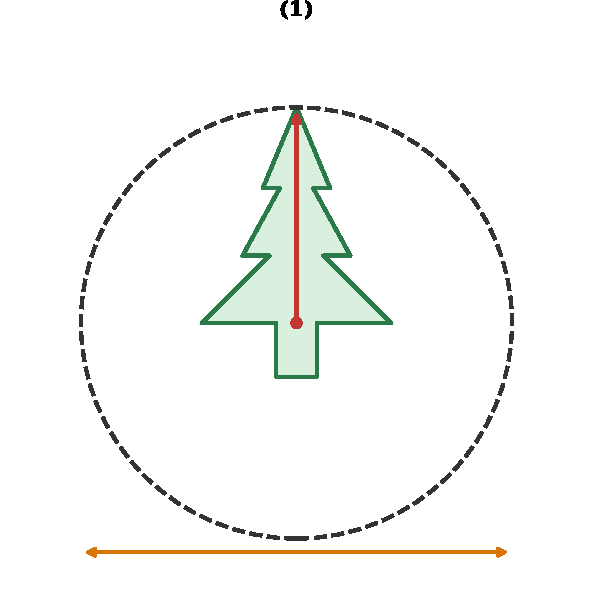
\includegraphics[width=\linewidth]{img/collision_panel_1}
  \end{minipage}
  \hfill
  \begin{minipage}[t]{0.49\linewidth}
    \centering
    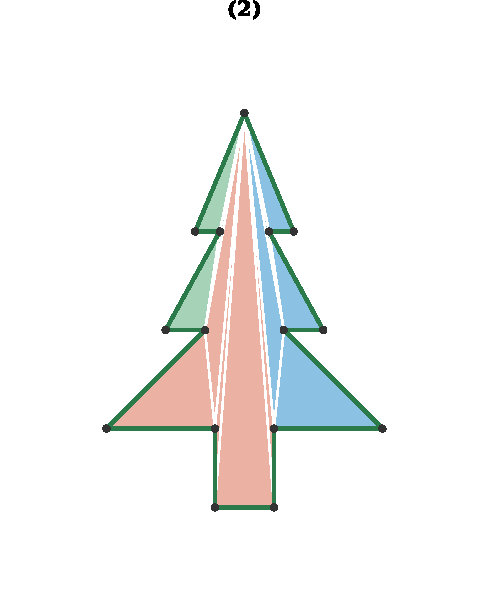
\includegraphics[width=\linewidth]{img/collision_panel_2}
  \end{minipage}

  \vspace{6pt}

  \begin{minipage}[t]{0.49\linewidth}
    \centering
    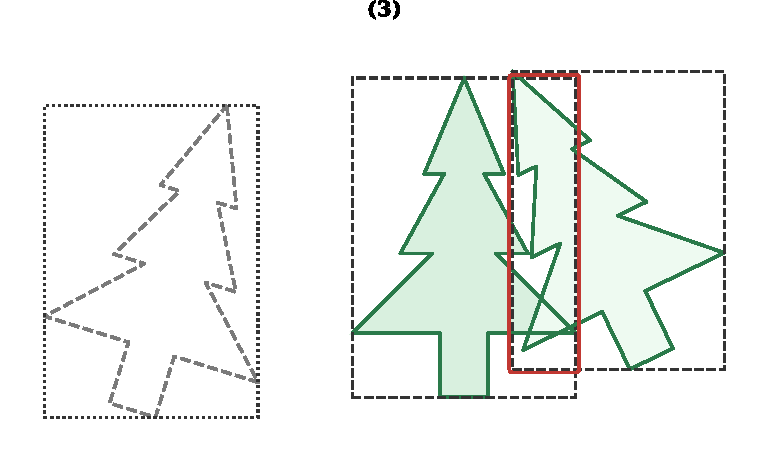
\includegraphics[width=\linewidth]{img/collision_panel_3}
  \end{minipage}
  \hfill
  \begin{minipage}[t]{0.49\linewidth}
    \centering
    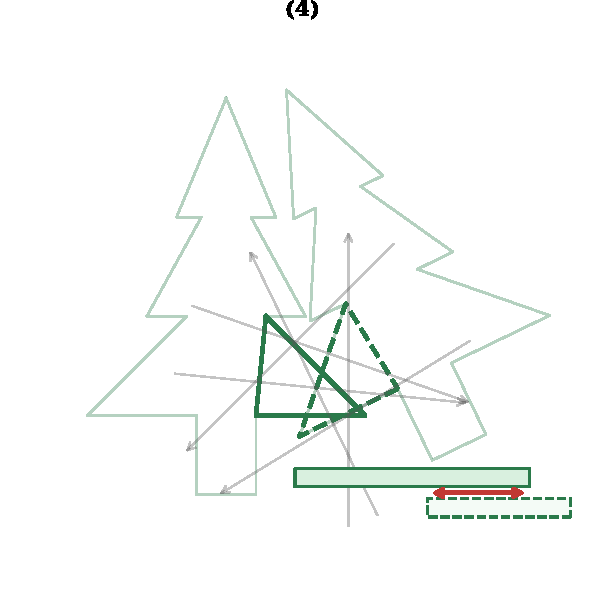
\includegraphics[width=\linewidth]{img/collision_panel_4}
  \end{minipage}

  \caption{Collision detection pipeline. Top-left: broad phase using a uniform spatial hash and neighborhood query. Top-right: polygon AABB culling. Bottom-left: group-level AABB pruning after triangulation into clustered subsets. Bottom-right: triangle-triangle SAT narrow phase returning penetration depth $d$, which feeds the overlap energy.}
  \label{fig:collision-pipeline}
  \vspace{4pt}
\end{figure}

Offline, the polygon is triangulated as a fan from vertex 0
 into $T = 13$ triangles. These are grouped into three clusters
  of sizes $(5, 5, 3)$ and cached as AABBs. 
  During narrow-phase evaluation, the SAT projects triangle pairs onto
   six edge-normal axes to compute the minimum overlap width,
    $d \geq 0$. World-space vertices are projected directly
     to avoid recomputing rotation matrices on each call.
      If a gap appears on any axis, the triangles are disjoint.
       Otherwise, $d > 0$ yields the penetration depth,
        providing a continuous measure of intersection severity.
         Relying on a binary collision penalty would create a flat
          energy landscape with no gradient. By contrast,
           the depth $d$ supplies a clear directional signal.
            Then, feeding $d^2$ into the energy function generates
             the smooth guidance necessary to steer the simmulated annealing 
             optimization toward feasibility from arbitrary
              starting states.



\subsection{Energy Function and Simmulated Annealing Schedule}
We model feasibility as a soft-constrained optimization problem, penalizing both 
geometric interpenetration and container boundary violations. 
The total energy of a configuration at container side length
 $L$ is$$E = \lambda \sum_{i<j}\;\sum_{(a,b)\in\mathcal{T}_{ij}}d(a,b)^{2} + \mu \sum_i \phi_i(L), \label{eq:energy}$$
 where $d(a,b)$ is the SAT penetration depth between triangle pair $(a, b)$, $\phi_i(L)$ is the squared AABB 
 boundary violation of copy $i$, and $(\lambda, \mu)$ are the respective penalty weights. A configuration
  is declared strictly feasible when the unweighted residual is negligible:
  $$\mathcal{F} = \sum_{i<j} \text{overlap}_{ij} + \sum_i \phi_i < 10^{-10}.$$To minimize $E$, the simmulated annealing trial 
  executes two sequential phases with geometrically decreasing temperature
   $T_k = T_0\,\beta^k$, where $\beta = (T_{\mathrm{end}}/T_0)^{1/M}$:Phase A (Exploration; 70{,}000 iterations): 
   Prioritizes broad search using a high initial temperature $T_0 = 0.30$ and a linear overlap penalty ($p = 1$).
   Phase B (Feasibility; 35{,}000 iterations): Drives the system toward strict feasibility 
   by dropping $T_0$ to $0.06$, switching to a quadratic penalty ($p = 2$), and scaling penalty weights by 
   a factor of 1.8 every 1{,}200 iterations.Throughout both phases, step sizes $(s_{xy}, s_\theta)$ 
   dynamically adapt every 1{,}500 iterations to maintain a target acceptance band, automatically coupling 
   the search radius to the cooling temperature. While small $N$ instances execute the full
    105{,}000-iteration budget, wall-clock limits may truncate Phase B for larger $N$. Table~\ref{tab:sa} 
    summarizes the schedule.




\begin{table}[t]
\centering\small
\setlength{\tabcolsep}{4.5pt}
\caption{Two-phase simmulated annealing schedule parameters.}
\label{tab:sa}
\begin{tabular}{lcc}
\toprule
Parameter & Phase A & Phase B \\
\midrule
Iterations $M$                & $70{,}000$       & $35{,}000$ \\
$T_{\mathrm{start}}$          & $0.30$           & $0.06$ \\
$T_{\mathrm{end}}$            & $3\times10^{-4}$ & $10^{-6}$ \\
Overlap power $p$             & 1                & 2 \\
$\lambda_0,\,\mu_0$           & $10^2$ (fixed)   & $10^3$ (ramped) \\
Step adapt window             & \multicolumn{2}{c}{$1{,}500$ iters} \\
Acceptance band               & $[0.25,\,0.55]$  & $[0.10,\,0.30]$ \\
Step shrink / grow            & $0.88$ / $1.12$  & $0.90$ / $1.08$ \\
Reinsertion prob.             & $2\%$            & $0.5\%$ \\
Feasibility $\mathcal{F} <$   & \multicolumn{2}{c}{$10^{-10}$} \\
\bottomrule
\end{tabular}
\end{table}

\subsection{Outer Loop: Bisection and Polish}

The simmulated annealing solver is used as a feasibility oracle at fixed
container side length $L$. The outer loop in the 2025 implementation first
builds a valid bracket, then runs fixed-count bisection, and finally performs
an adaptive long-run polish.

Bracketing does not start directly from
$[L_{\mathrm{area}},\,\gamma L_{\mathrm{area}}]$.
Instead, the run starts from a grid-based initial layout and tests feasibility.
If that state is feasible, the solver repeatedly shrinks $L$ until infeasible;
if infeasible, it grows $L$ until feasible.
This yields a bracket $[L_{\mathrm{low}}, L_{\mathrm{high}}]$ with
$L_{\mathrm{low}}$ infeasible and $L_{\mathrm{high}}$ feasible.

The lower side is anchored by a provable area bound,
$L_{\mathrm{area\_infeas}}=\sqrt{N A_p}(1-10^{-9})$.
Values at or below this bound are treated as provably infeasible.
During bisection, the midpoint
$L_{\mathrm{mid}}=\tfrac{1}{2}(L_{\mathrm{low}}+L_{\mathrm{high}})$
is tested with SA:
feasible updates $L_{\mathrm{high}}\leftarrow L_{\mathrm{mid}}$,
infeasible updates $L_{\mathrm{low}}\leftarrow L_{\mathrm{mid}}$.
The 2025 code performs a fixed 26 bisection iterations.

Warm starts are used throughout: when $L$ changes, polygon centers are rescaled
from the previous feasible layout before launching the next SA call.
This preserves geometric structure and significantly reduces re-equilibration time.

\textbf{Bisection + warm-start pseudocode}
\begin{enumerate}[leftmargin=1.2em]
  \item Build bracket by shrink/grow passes from a grid-initialized state:
        find infeasible $L_{\mathrm{low}}$ and feasible $L_{\mathrm{high}}$.
  \item For $k=1,\dots,26$:
    \begin{enumerate}[leftmargin=1.4em]
      \item $L_{\mathrm{mid}}\leftarrow \tfrac{1}{2}(L_{\mathrm{low}}+L_{\mathrm{high}})$.
      \item If $L_{\mathrm{mid}} \le L_{\mathrm{area\_infeas}}$, set
            $L_{\mathrm{low}}\leftarrow L_{\mathrm{mid}}$ and continue.
      \item Warm-start by scaling centers from previous feasible $L$ to $L_{\mathrm{mid}}$.
      \item Run SA at $L_{\mathrm{mid}}$.
      \item If feasible: set $L_{\mathrm{high}}\leftarrow L_{\mathrm{mid}}$ and save state.
      \item Else: set $L_{\mathrm{low}}\leftarrow L_{\mathrm{mid}}$.
    \end{enumerate}
\end{enumerate}

\textbf{Polish-stage pseudocode}
\begin{enumerate}[leftmargin=1.2em]
  \item Start from post-bisection best feasible state $(L^*,\mathcal{C}^*)$.
  \item Maintain adaptive shrink factor $\varepsilon$ and a rolling window of 20 attempts.
  \item Repeatedly propose $L_{\mathrm{try}}=L^*(1-\varepsilon)$, warm-start, and run SA.
  \item On success: accept $L_{\mathrm{try}}$, update $(L^*,\mathcal{C}^*)$.
  \item Every 20 attempts, compare success rate to the 35\% target and adapt $\varepsilon$.
  \item Flush checkpoints periodically and on \texttt{SIGTERM}.
\end{enumerate}

After bisection, an adaptive polish phase progressively shrinks the
container: at each attempt the solver tries $L \leftarrow L^*(1 -
\varepsilon)$ with $\varepsilon$ adapted over rolling windows of 20
probes to maintain a target success rate of roughly 35\%, then runs SA
at the candidate $L$. A successful packing updates the best known
$L^*$. Artifacts confirm this phase produces repeated improvements in
$L$ over time, and it accounts for the majority of density gain at
large $N$. Progress is written to disk on every improvement, and a
global snapshot is flushed on \texttt{SIGTERM} so SLURM preemption
loses no work. Every worker is seeded deterministically from (base
seed, run ID, trial index) via SplitMix64, guaranteeing full
reproducibility.
% ================================================================
\section{Experimental Setup}
\label{sec:experiments}

All computational experiments were conducted on the University of
 Arizona high-performance computing (HPC) cluster.
  The results reported herein derive from
   \emph{single-node SLURM array jobs}.
    Each array task executed a single independent random seed,
     with a maximum of two seeds running concurrently per job. 
     We configured the array sizes and wall-clock limits according 
     to the problem size: 8 tasks at $N = 25$ 
     (4-hour wall time, yielding an effective search budget of
      14{,}100,s after a 300-second post-processing cushion),
       6 tasks at $N = 50$ (4,h), 4 tasks at $N = 100$ (4,h),
        and 2 tasks at $N = 200$ (8,h wall time, yielding a
         28{,}500,s effective budget). To ensure data integrity,
          SLURM was configured to send a \texttt{SIGTERM}
           signal 120,s prior to the hard time limit, allowing the solver
            sufficient time to flush its best-found snapshot to disk.
             Because these runs executed without inter-worker communication,
              the global best solution for each instance of $N$
               was identified through
 a post-hoc reduction pass over all resulting output CSV files.
% ================================================================
\section{Results}
\label{sec:results}

We first inspect the best feasible side-length trajectories over wall time,
then the final recovered packing configurations, and then a cross-$N$
summary of the best feasible side lengths.

\begin{figure}[!tbp]
  \centering
  {\bfseries Best Feasible Side Length Over Time (Small N)\par}
  \vspace{4pt}
  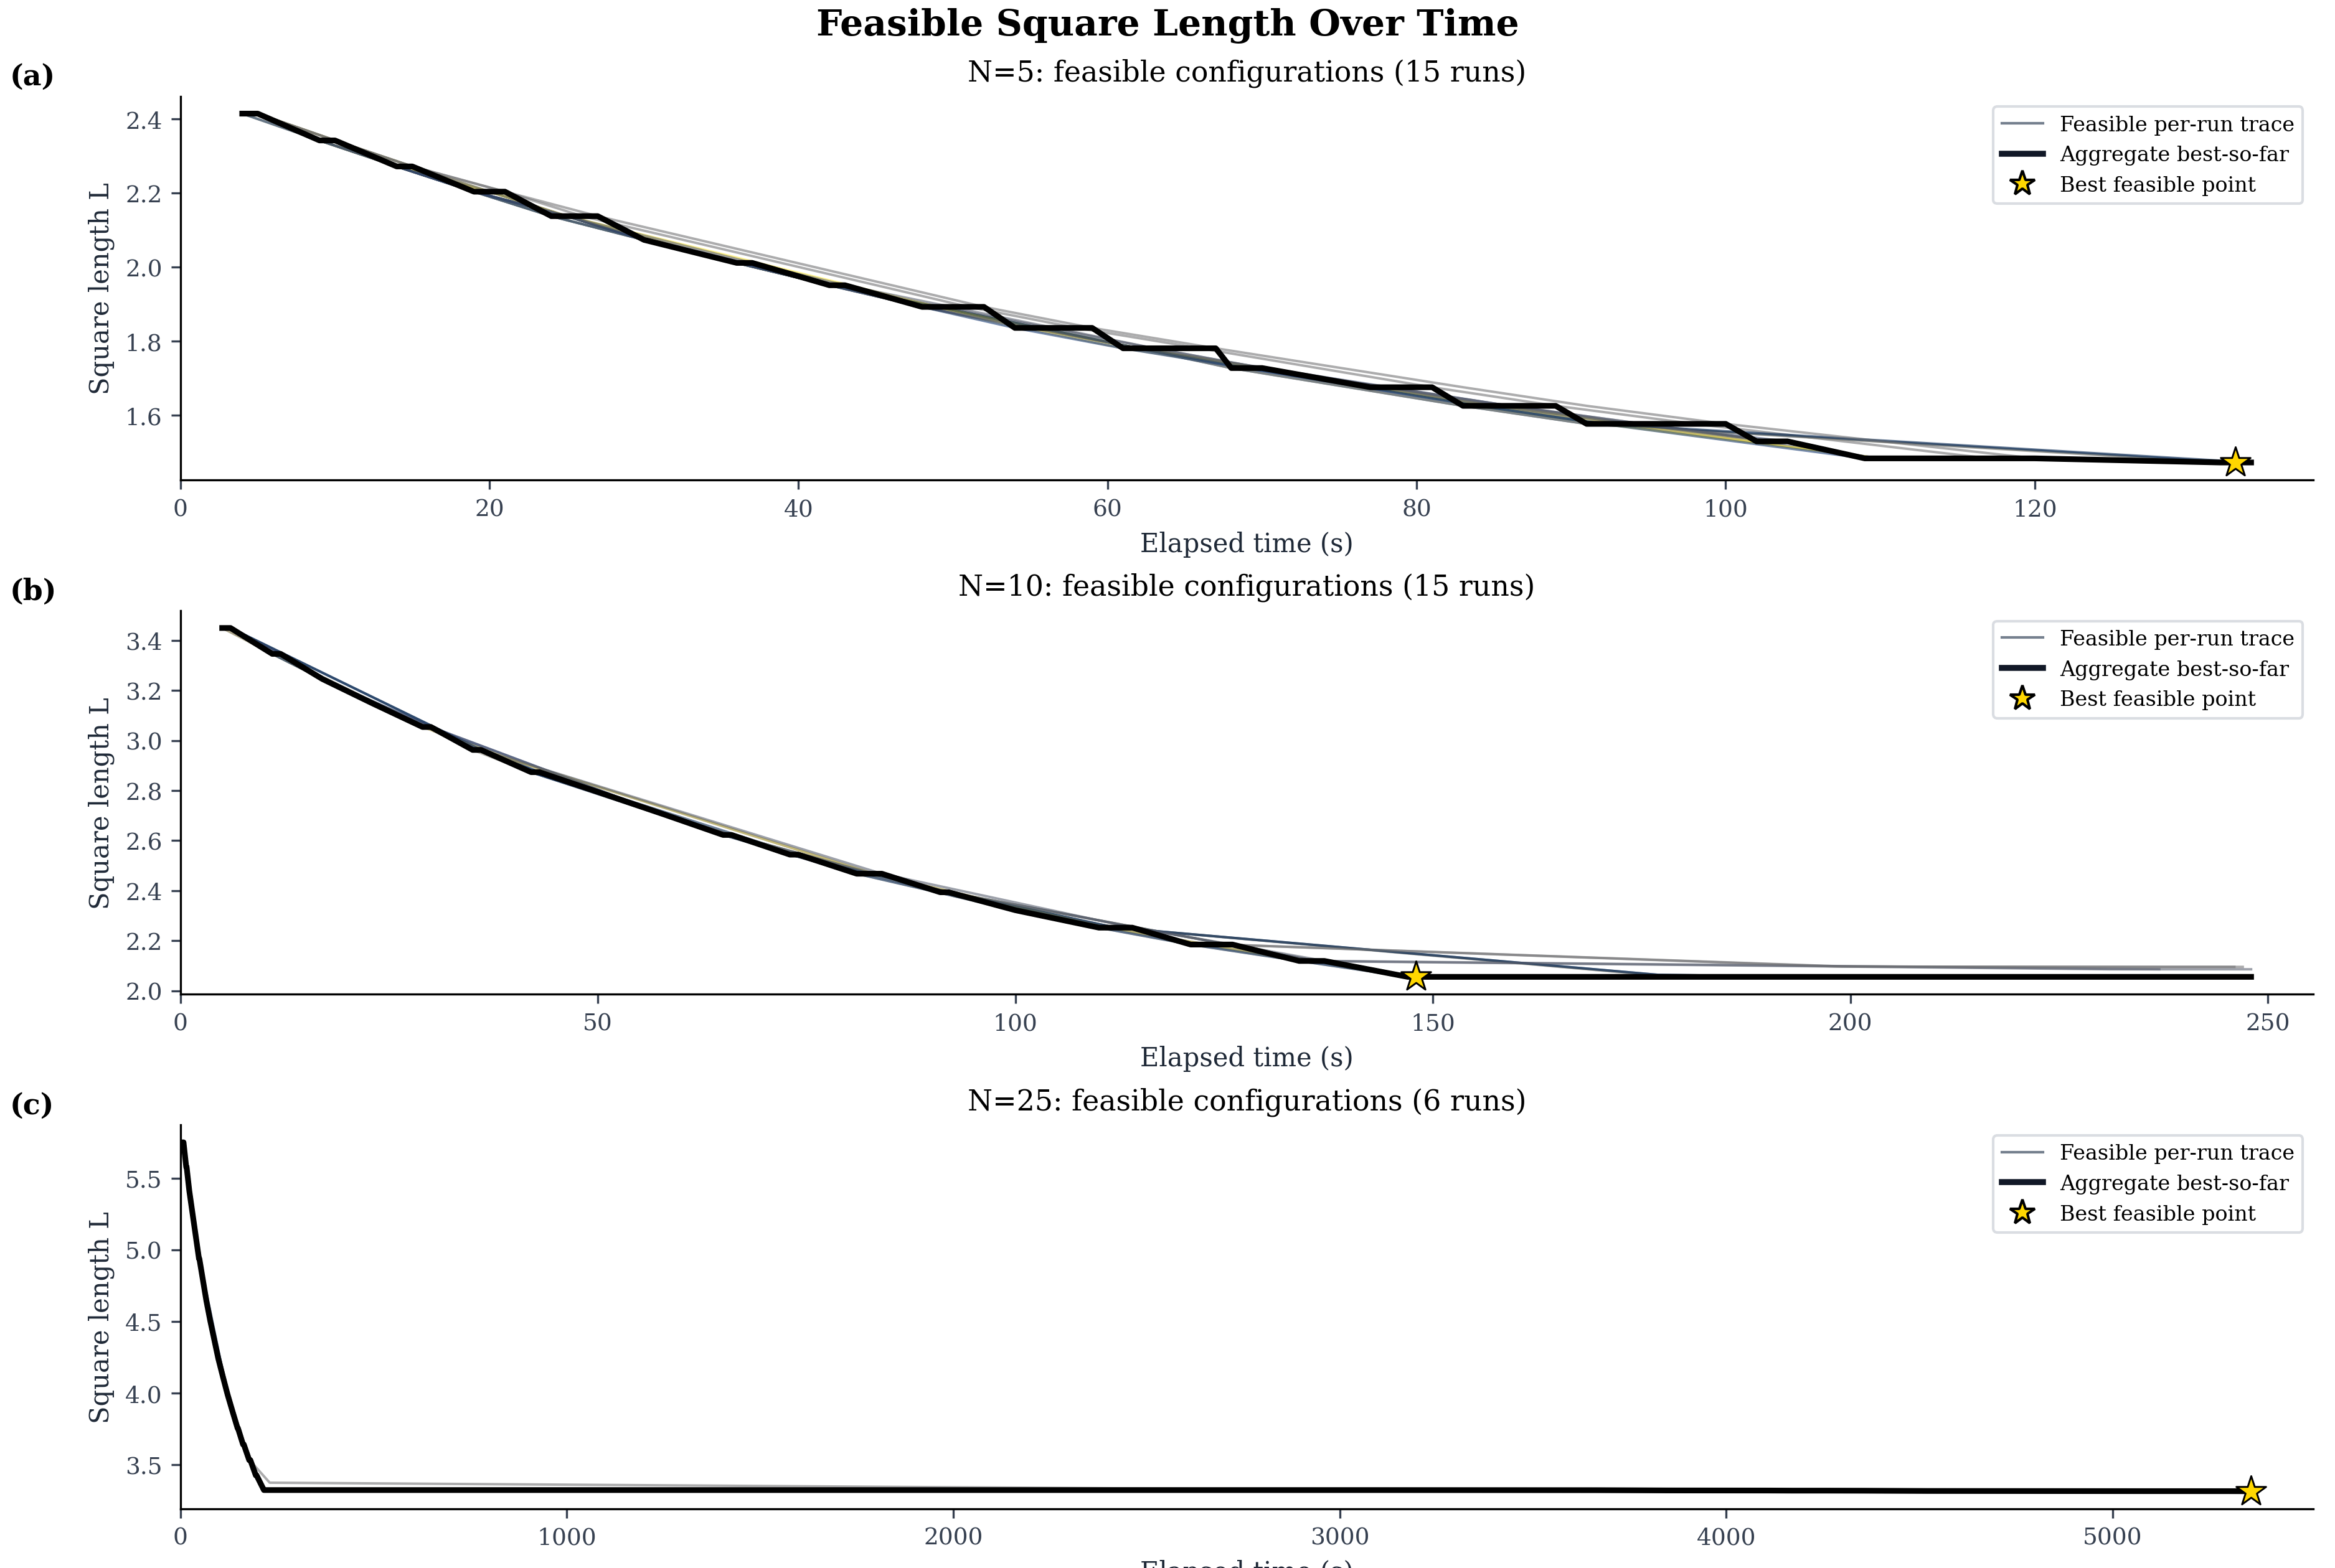
\includegraphics[width=\linewidth]{img/feasible_L_timeseries_N5_N10_N25.png}
  \caption{Best-so-far feasible square side length $L$ versus wall time for $N \in \{5,10,25\}$.}
  \label{fig:timeseries-smallN}
  \vspace{4pt}
\end{figure}


\begin{figure}[!tbp]
  \centering
  {\bfseries Final Best Configurations by Instance Size\par}
  \vspace{4pt}

  \begin{minipage}[t]{0.48\linewidth}
    \centering
    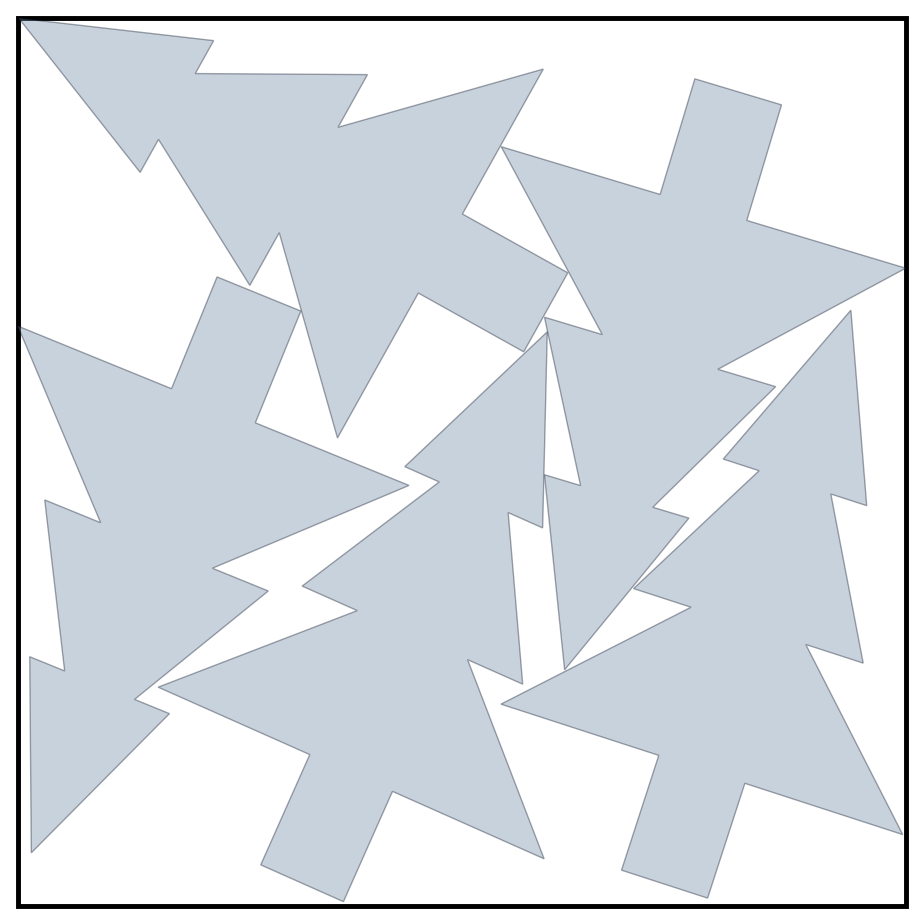
\includegraphics[width=\linewidth,height=0.22\textheight,keepaspectratio]{img/per_n_configs/N005_best_config.png}
    \small $N=5$
  \end{minipage}
  \hfill
  \begin{minipage}[t]{0.48\linewidth}
    \centering
    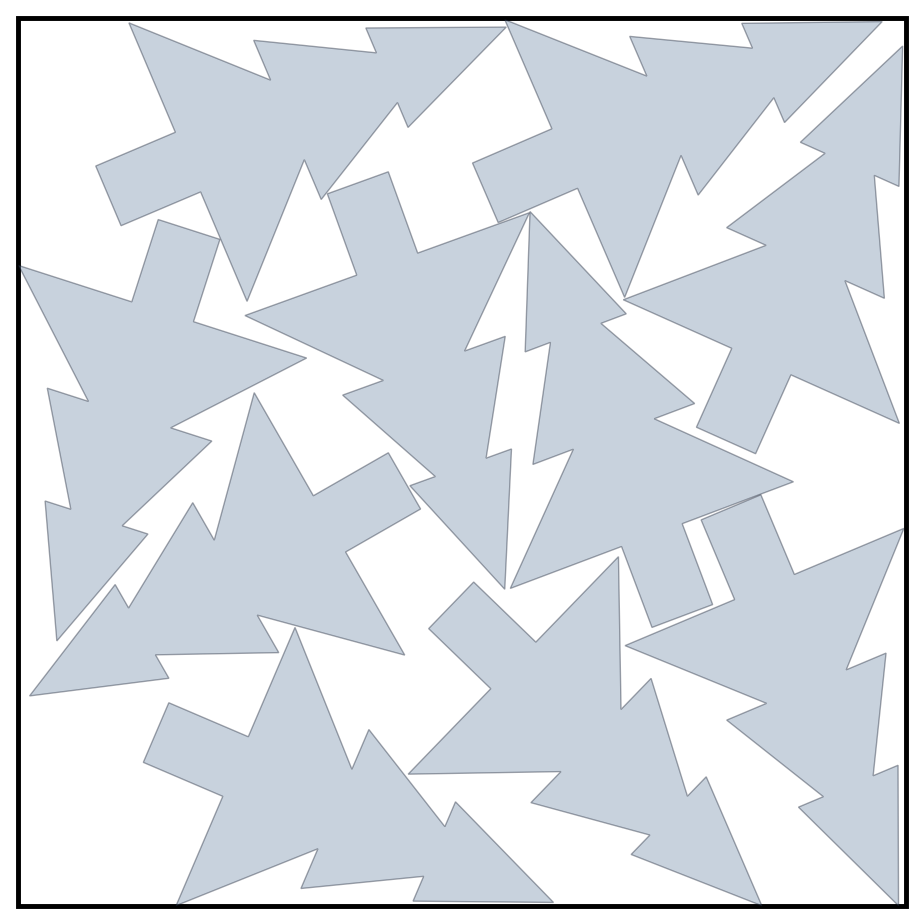
\includegraphics[width=\linewidth,height=0.22\textheight,keepaspectratio]{img/per_n_configs/N010_best_config.png}
    \small $N=10$
  \end{minipage}

  \vspace{6pt}

  \begin{minipage}[t]{0.48\linewidth}
    \centering
    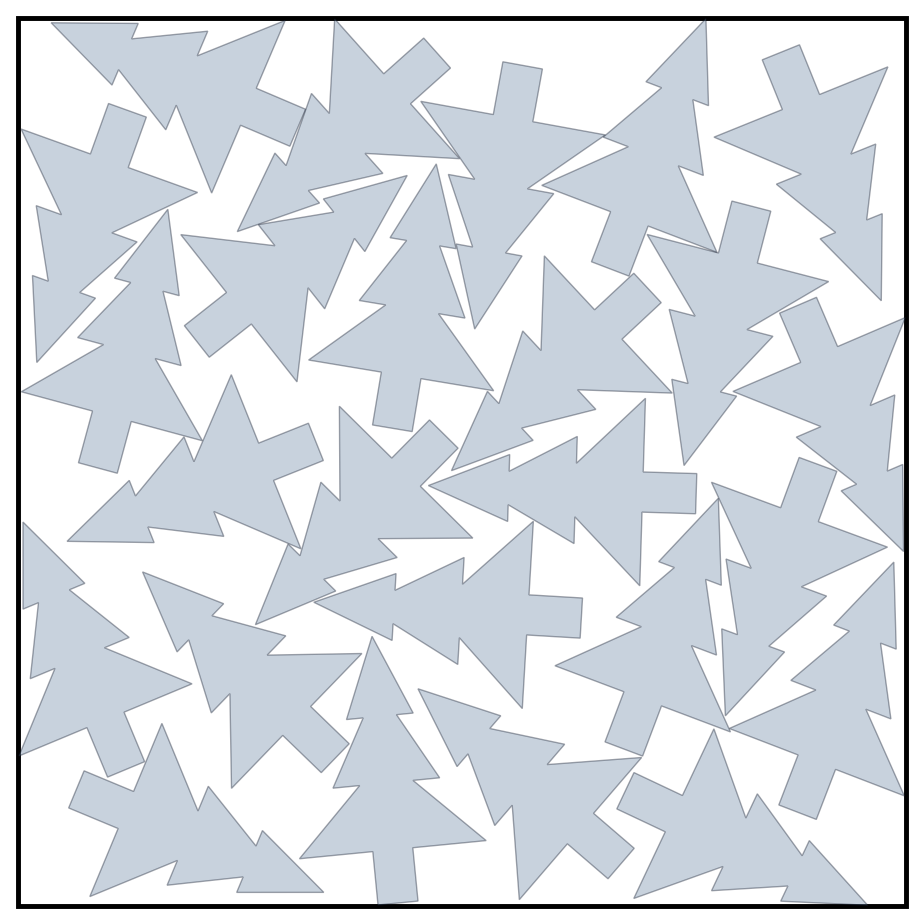
\includegraphics[width=\linewidth,height=0.22\textheight,keepaspectratio]{img/per_n_configs/N025_best_config.png}
    \small $N=25$
  \end{minipage}
  \hfill
  \begin{minipage}[t]{0.48\linewidth}
    \centering
    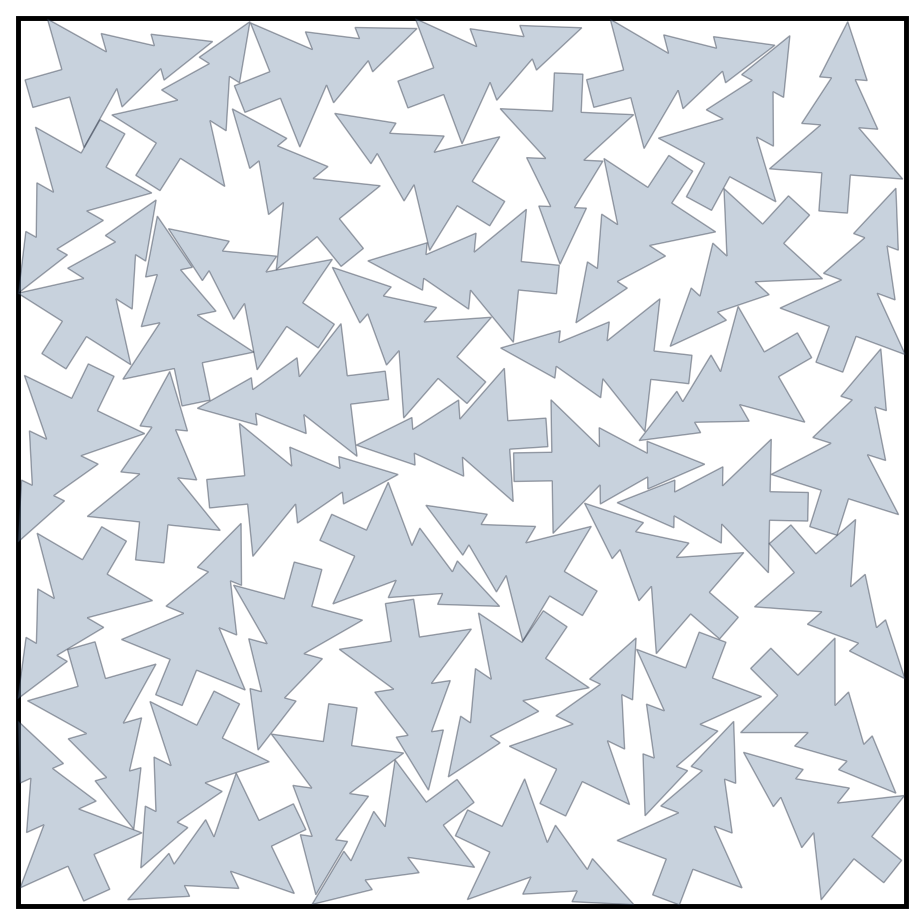
\includegraphics[width=\linewidth,height=0.22\textheight,keepaspectratio]{img/per_n_configs/N050_best_config.png}
    \small $N=50$
  \end{minipage}

  \vspace{6pt}

  \begin{minipage}[t]{0.48\linewidth}
    \centering
    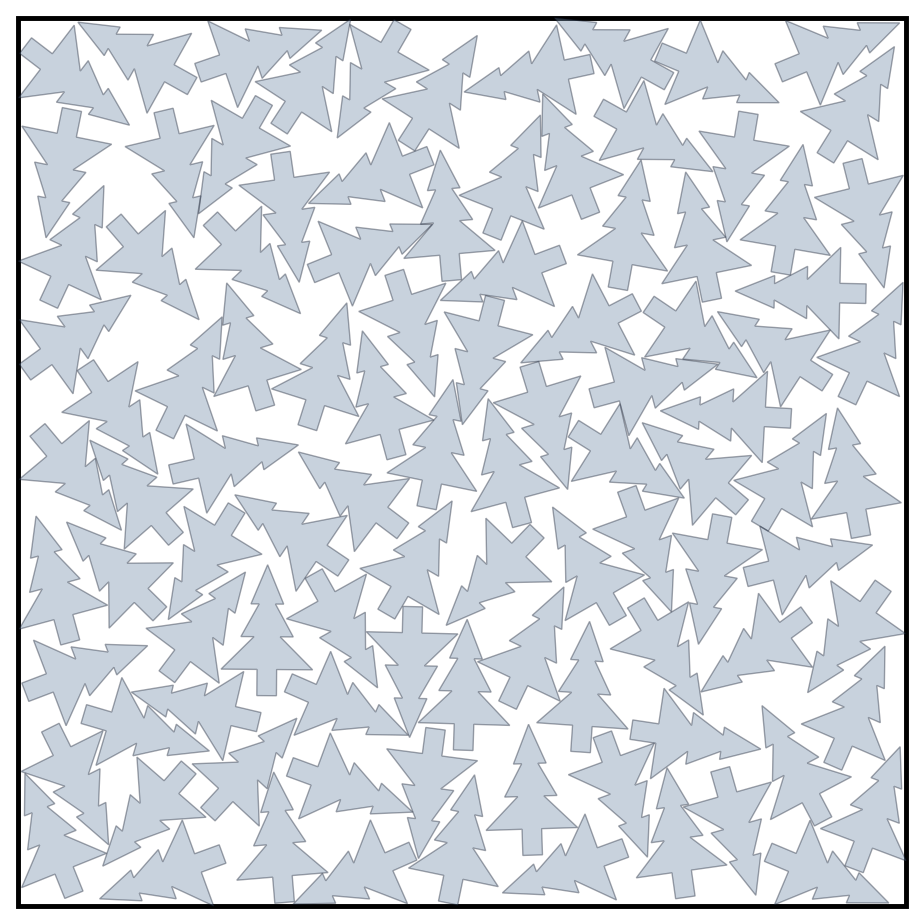
\includegraphics[width=\linewidth,height=0.22\textheight,keepaspectratio]{img/per_n_configs/N100_best_config.png}
    \small $N=100$
  \end{minipage}
  \hfill
  \begin{minipage}[t]{0.48\linewidth}
    \centering
    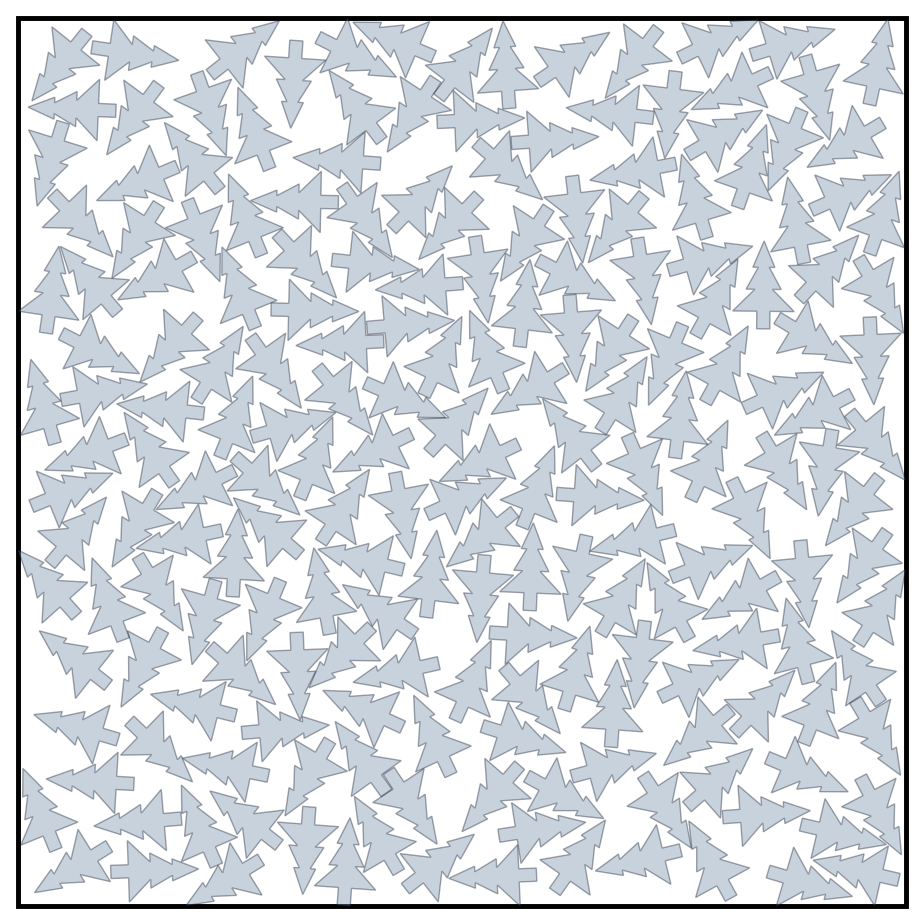
\includegraphics[width=\linewidth,height=0.22\textheight,keepaspectratio]{img/per_n_configs/N200_best_config.png}
    \small $N=200$
  \end{minipage}

  \caption{Best recovered polygon packing configurations for each reported problem size.}
  \label{fig:final-configs-allN}
  \vspace{4pt}
\end{figure}




\begin{figure}[!htbp]
  \centering
  {\bfseries Best Feasible Side Length Over Time (Large N)\par}
  \vspace{4pt}
  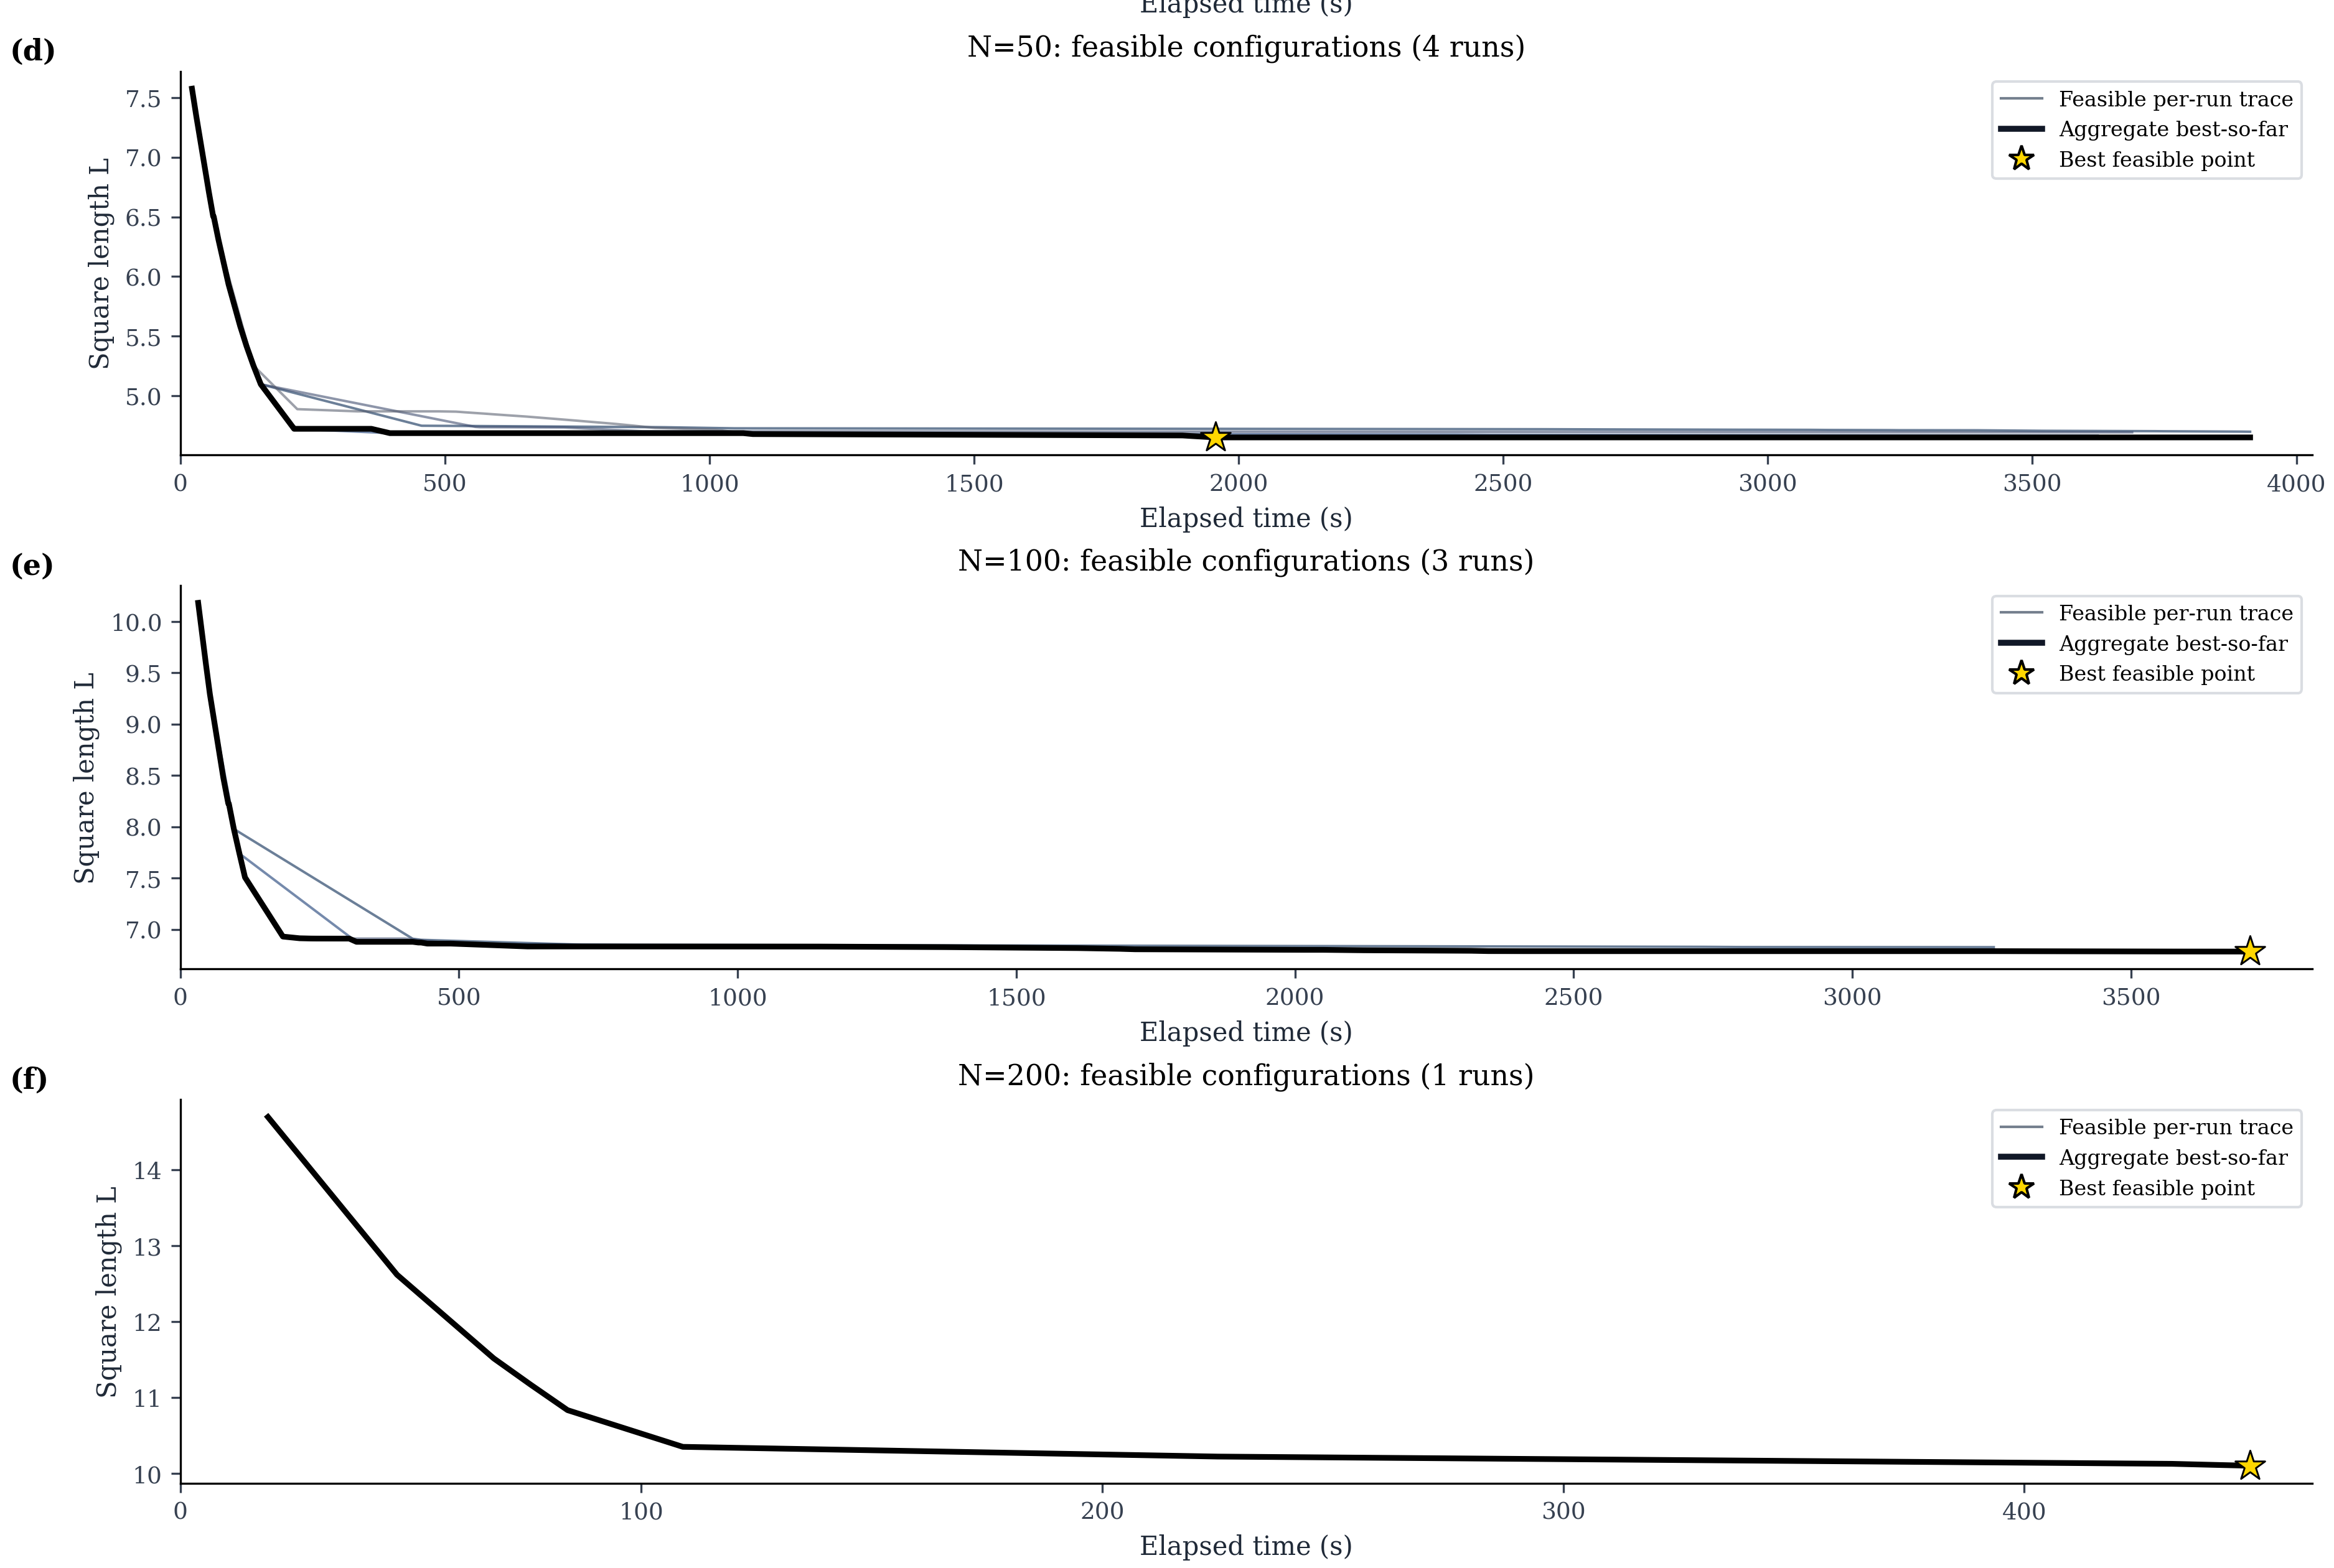
\includegraphics[width=\linewidth]{img/feasible_L_timeseries_N50_N100_N200.png}
  \caption{Best-so-far feasible square side length $L$ versus wall time for $N \in \{50,100,200\}$.}
  \label{fig:timeseries-largeN}
  \vspace{4pt}
\end{figure}


Table~\ref{tab:results} reports the best feasible side length $L^*$
and packing efficiency $\eta = N A_p / (L^*)^2$ for each $N$. The
area lower bound $L_{\mathrm{area}} = \sqrt{N A_p}$ is given for
reference; $\eta = 1$ would require zero wasted space, which is
geometrically impossible for this non-convex shape. The column
``Runs'' counts workers that found at least one feasible configuration.

\begin{table}[!tbp]
\centering\small
\setlength{\tabcolsep}{3.5pt}
\caption{Best feasible side length, packing efficiency, and
feasibility rate by instance size. $N = 5$ and $N = 10$ used the
five-node pipeline (3-min smoke tests); $N \geq 25$ used single-node
array jobs (4--8\,h). Cross-$N$ comparisons should be read with this
provenance difference in mind.}
\label{tab:results}
\begin{tabular}{r@{\hskip6pt}ccccc}
\toprule
$N$ & $L_{\mathrm{area}}$ & $L^*$ & $\eta$ & Runs &
$t_{\mathrm{first}}$ \\
\midrule
  5 & 1.108 & 1.472 & 0.567 & 15 &  5\,s \\
 10 & 1.568 & 2.056 & 0.581 & 15 &  6\,s \\
 25 & 2.478 & 3.315 & 0.559 &  6 &  8\,s \\
 50 & 3.504 & 4.652 & 0.567 &  4 & 46\,s \\
100 & 4.956 & 6.785 & 0.533 &  3 & 53\,s \\
200 & 7.009 & 10.104& 0.481 &  1 & 19\,s \\
\bottomrule
\end{tabular}
\end{table}

Observe three patterns emerge. First, the number of workers reaching
feasibility drops sharply: 15 of 15 at $N = 5$ and $N = 10$, down to
6 at $N = 25$, and to a single run at $N = 200$. The simulated annealing is
time-budgeted and not iteration-bounded, but the cost per simulated annealing proposal
grows with $N$ since more polygon pairs must be checked. At large
$N$ we can fit fewer trials within the wall-time budget, and the trials that
do run explore a configuration space of dimension $3N$ with
proportionally less coverage per polygon. The configuration space at
$N = 200$ has 600 degrees of freedom.

Second, the best feasible side length increases monotonically with
$N$, while the gap between $L^*$ and the area lower bound remains substantial across all tested
sizes. The final packings in Figure~\ref{fig:final-configs-allN}
show this increasingly constrained geometry directly: larger instances
still admit feasible layouts, but with visibly tighter global packing
structure and less slack for local rearrangement.

Third, the median time to final best configuration was 205\,s at
$N = 25$ but exceeded 3{,}250\,s at $N = 100$, out of a 14{,}100\,s
budget. Most improvement arrived at 23--26\% into the run, confirming
that the polish phase, not the bisection loop, produces the majority
of the density gain at large $N$. At small $N$ the bisection alone is
nearly sufficient; at large $N$ the bulk of the productive computation
happens during extended feasibility polish.


\clearpage

% ================================================================
\section{Conclusion}
\label{sec:conclusion}

The interestiing aspect of our apporach was the use of 
the Separating Axis Theorem (SAT) to measure penetration depth rather
than relying on a binary collision test. This allowed us to craft an energy
function that allows for states with some overlap and a continuous penalty that guides the
Simulated Annealing algorithm out of messy, heavily overlapping
starting states and into strictly feasible packings. 

We observe most of the gains in a configuration were achieved during the adaptive polish phase. 
Once the outer
bisection loop rapidly narrowed down the target container size $L^*$,
the adaptive polish phase did the heavy lifting, squeezing out the
majority of the final density gains.

However, our HPC experiments revealed a fundamental bottleneck. As the
number of polygons $N$ increases, the computational cost of collision
checking grows so large that our time-budgeted runs could no longer
adequately explore the high-dimensional search space, causing the
success rate to collapse.

The primary contribution of this study is therefore strategic: in a
geometric landscape this rugged and fragmented, trial \emph{diversity}
matters vastly more than trial \emph{duration}. Letting a single
simulation run for hours will yield rapidly diminishing returns the moment
it gets trapped in a deep local minimum. Although we have some wiggle room
for overlap penalties, in packings with large $N$ our budget might not be enough
to find a better rearrengement so an update rule for the penalty budget is needed.
A much smarter and effective way to reduce this bottleneck is to launch many short,
 independent screening runs, dedicating continued compute time only 
 to the most promising states. This is a natural fit for GPU architecture,
  which excels at running large batches of independent trials in parallel.
   By massively scaling the number of parallel trials, we can maintain a high
    level of structural diversity in the search process, increasing the chances
     of finding high-quality packings even in the face of an exponentially growing
      configuration space.




Future work must operationalize this lesson. First
compute or measure the average time to get a sound packing.
Within this time budget run as many independent trials as possible, and then select the best ones
for continued refinement. Second, integrating
population-based methods such as parallel tempering or genetic
recombination would organically maintain the structural diversity
that serial Simulated Annealing lacks. Finally, while porting this
solver to a GPU architecture remains highly valuable, its true power
will lie in massively scaling the  volume of independent parallel
trials.

% ================================================================
\bibliographystyle{plain}
\begin{thebibliography}{8}

\bibitem{bennell2008}
J.~A. Bennell and J.~F. Oliveira.
The geometry of nesting problems: A tutorial.
\textit{Eur.\ J.\ Oper.\ Res.}, 184(2):397--415, 2008.

\bibitem{burke2006}
E.~K. Burke, G.~Kendall, and G.~Whitwell.
A new placement heuristic for the orthogonal stock-cutting problem.
\textit{Oper.\ Res.}, 52(4):655--671, 2004.

\bibitem{kaggle2025}
Kaggle.
Santa 2025 competition: Christmas Tree Packing Challenge.
\textit{kaggle.com/competitions/santa-2025}, 2025.

\bibitem{kirkpatrick1983}
S.~Kirkpatrick, C.~D. Gelatt, and M.~P. Vecchi.
Optimization by simulated annealing.
\textit{Science}, 220(4598):671--680, 1983.

\bibitem{leung2003}
T.~W. Leung, C.~K. Chan, and M.~D. Troutt.
Application of a mixed simulated annealing-genetic algorithm heuristic
for the two-dimensional orthogonal packing problem.
\textit{Eur.\ J.\ Oper.\ Res.}, 145(3):530--542, 2003.

\bibitem{sokal1997}
A.~Sokal.
Monte Carlo methods in statistical mechanics: Foundations and new algorithms.
In \textit{Functional Integration}, pages 131--192. Springer, 1997.

\bibitem{vogel2026}
T.~Vogel and Y.~W. Li.
Accelerating multicanonical sampling with irreversibility.
\textit{arXiv preprint arXiv:2601.18980}, 2026.

\bibitem{zhang2025}
L.~Zhang, P.~Potaptchik, J.~He, Y.~Du, A.~Doucet, F.~Vargas, H.-D. Dau, and S.~Syed.
Accelerated parallel tempering via neural transports.
\textit{arXiv preprint arXiv:2502.10328}, 2025.

\end{thebibliography}

% ================================================================
\appendix
\section{Appendix: Density Trajectory}
\label{sec:appendix-density}

\begin{figure}[!htbp]
  \centering
  {\bfseries Best Density Over Time\par}
  \vspace{4pt}
  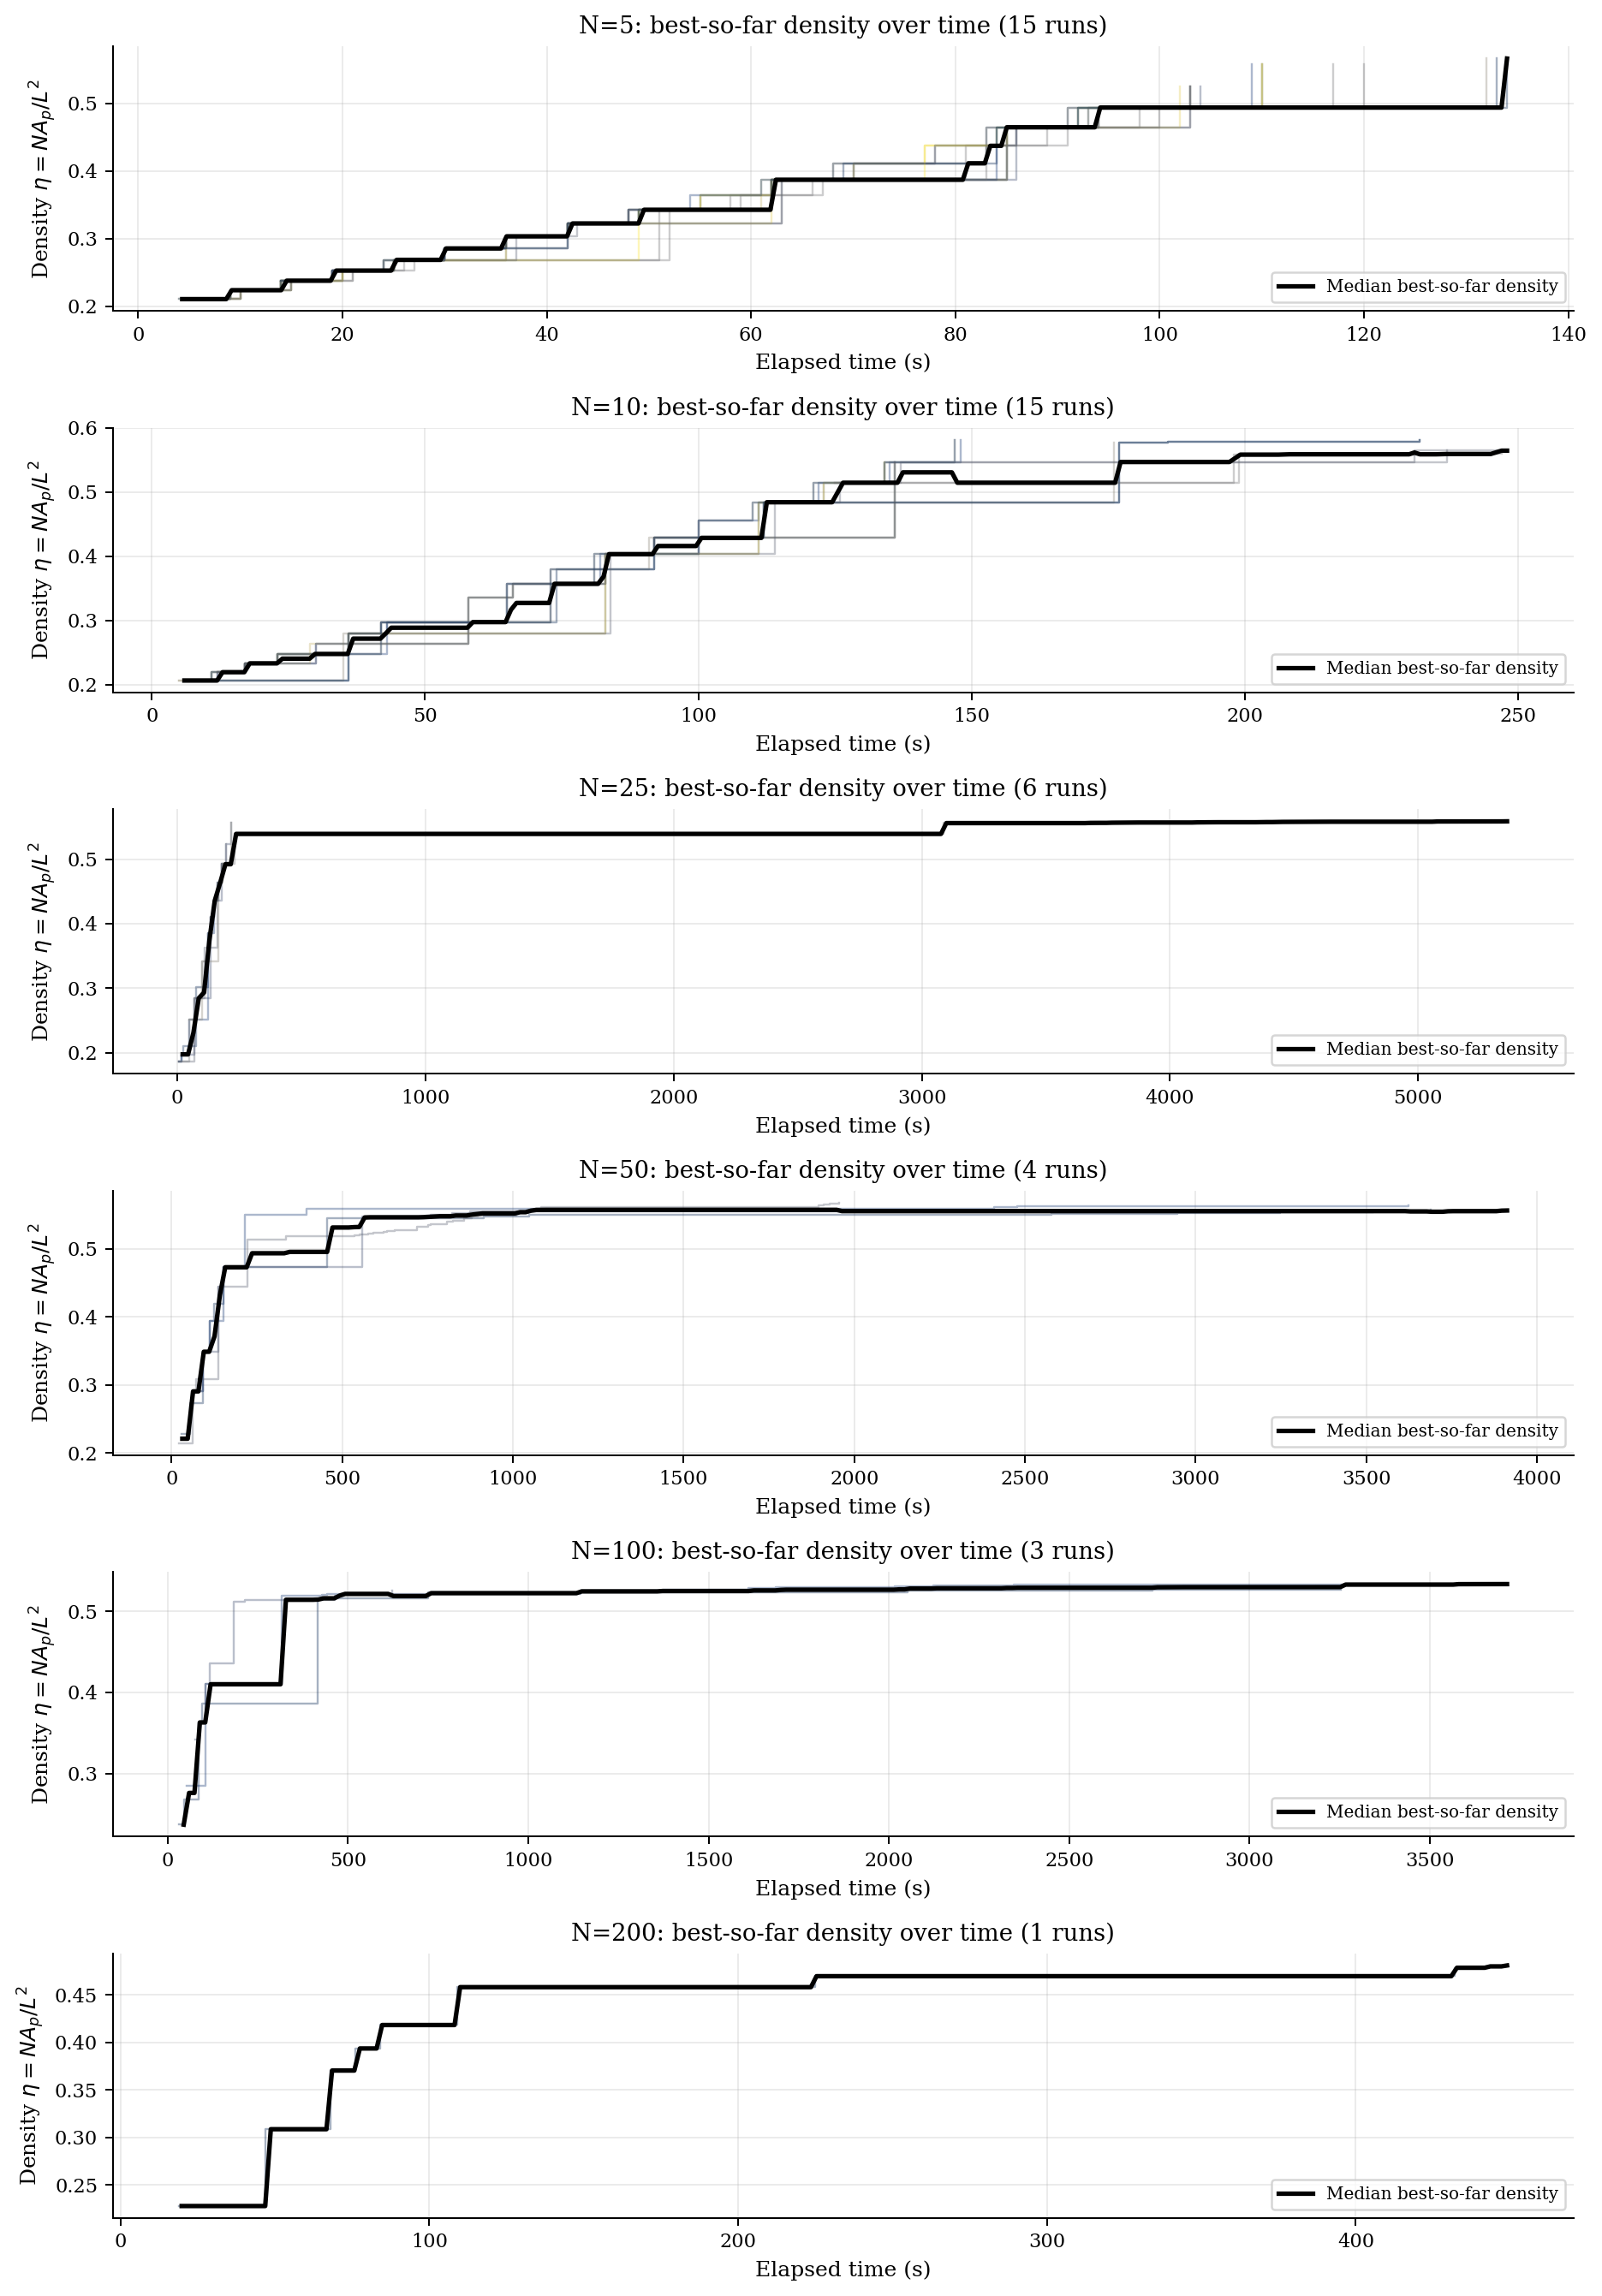
\includegraphics[width=\linewidth,height=0.68\textheight,keepaspectratio]{img/feasible_best_density_timeseries.png}
  \caption{Best-so-far packing density $\eta = N A_p/L^2$ versus wall time. The late-time slope at larger $N$ is consistent with most of the final improvement occurring during feasibility polish rather than during the initial bracket search.}
  \label{fig:density-full}
  \vspace{4pt}
\end{figure}
\end{document}
